\section{User Documentation}
\textit{(This section is also part of the readme.md on the weekme-github repository)} \\
\\Using \textbf{WeekMe} you can plan your next week. Not more, not less. No bloated UI nor functions you will probably never use anyway. 
How does this \textbf{awesome application} work? Hopefully it's so intuitive that any explanation is unnecessary, but just in case here is a short introduction for you.

\subsection{Account}
Like in most web apps you can sign up for an account, log in and out as well as change your password and email. And of course there is also a solution in case you forget your password. 
\begin{figure}[H] 
	\centering 
	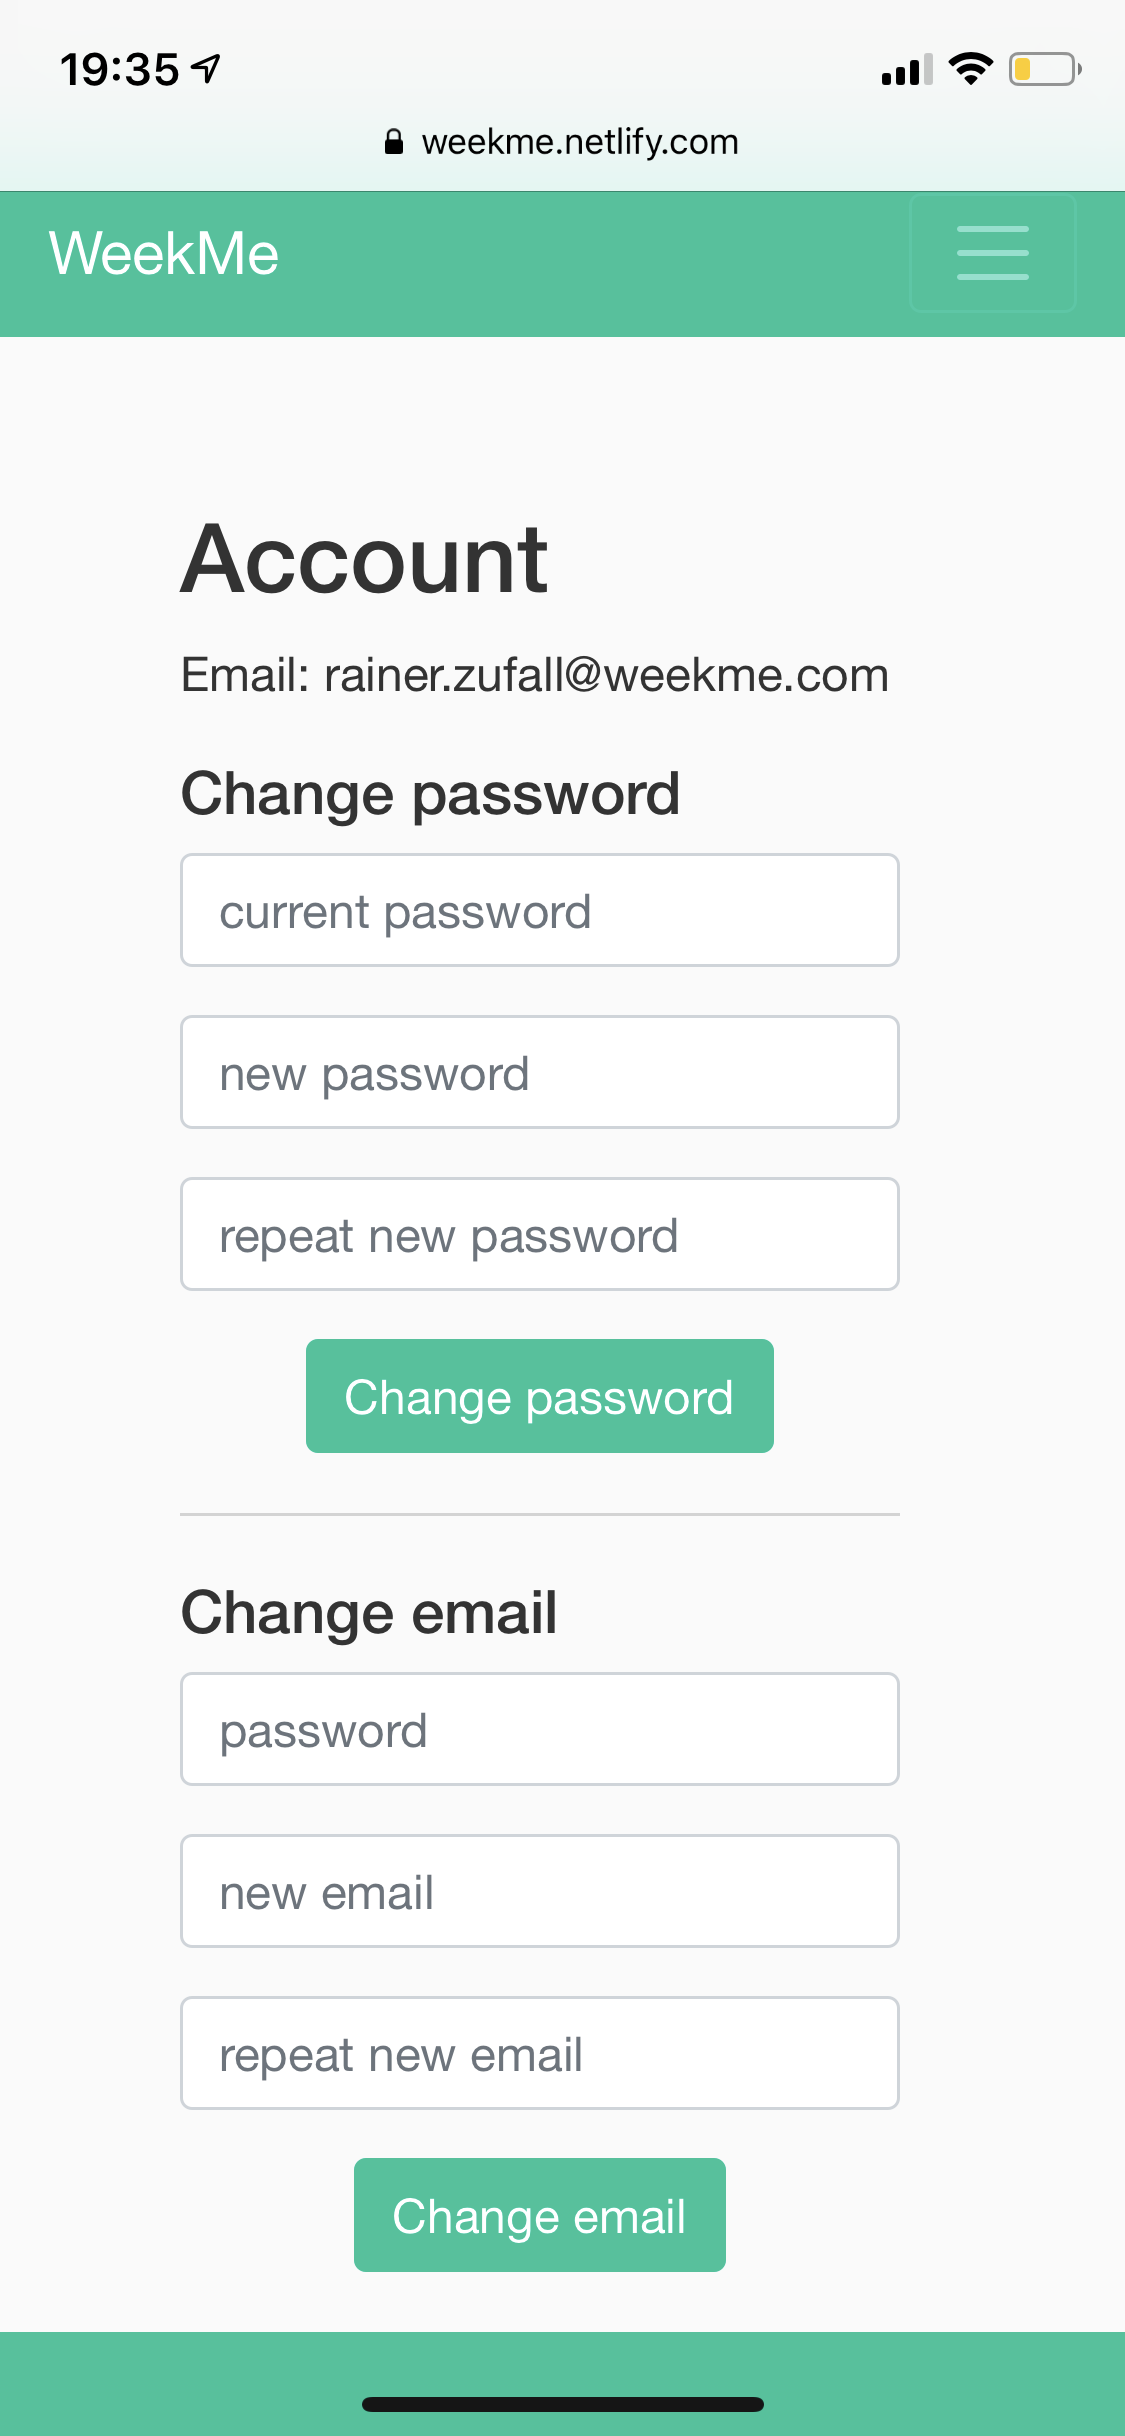
\includegraphics[height=10cm]{figures/user_docu_accounts_page.PNG}   
	\caption[WeekMe account page]{WeekMe account page on an iPhone XS}       
	\label{fig: Setting an environment variable in Heroku}     
\end{figure}  

\subsection{Working with tasks}
Since the app is all about planing your next weeks task, let's show you how you can work with these tasks on WeekMe. 
\subsubsection{Creating tasks}
To create a new task you select the plus icon where you want to add the task. This will bring up a popup window where you can enter a short description (up to 80 characters). 
If you fancy selecting a colour for your task to help you categorise, prioritise or just because you want more colour in your life - no false modesty, go on. Do it. 
In case you changed your mind or just clicked the wrong add button you can also change the day the task will be added to. 

\begin{figure}
    \centering
    \subfloat[Popup to enter description in]{{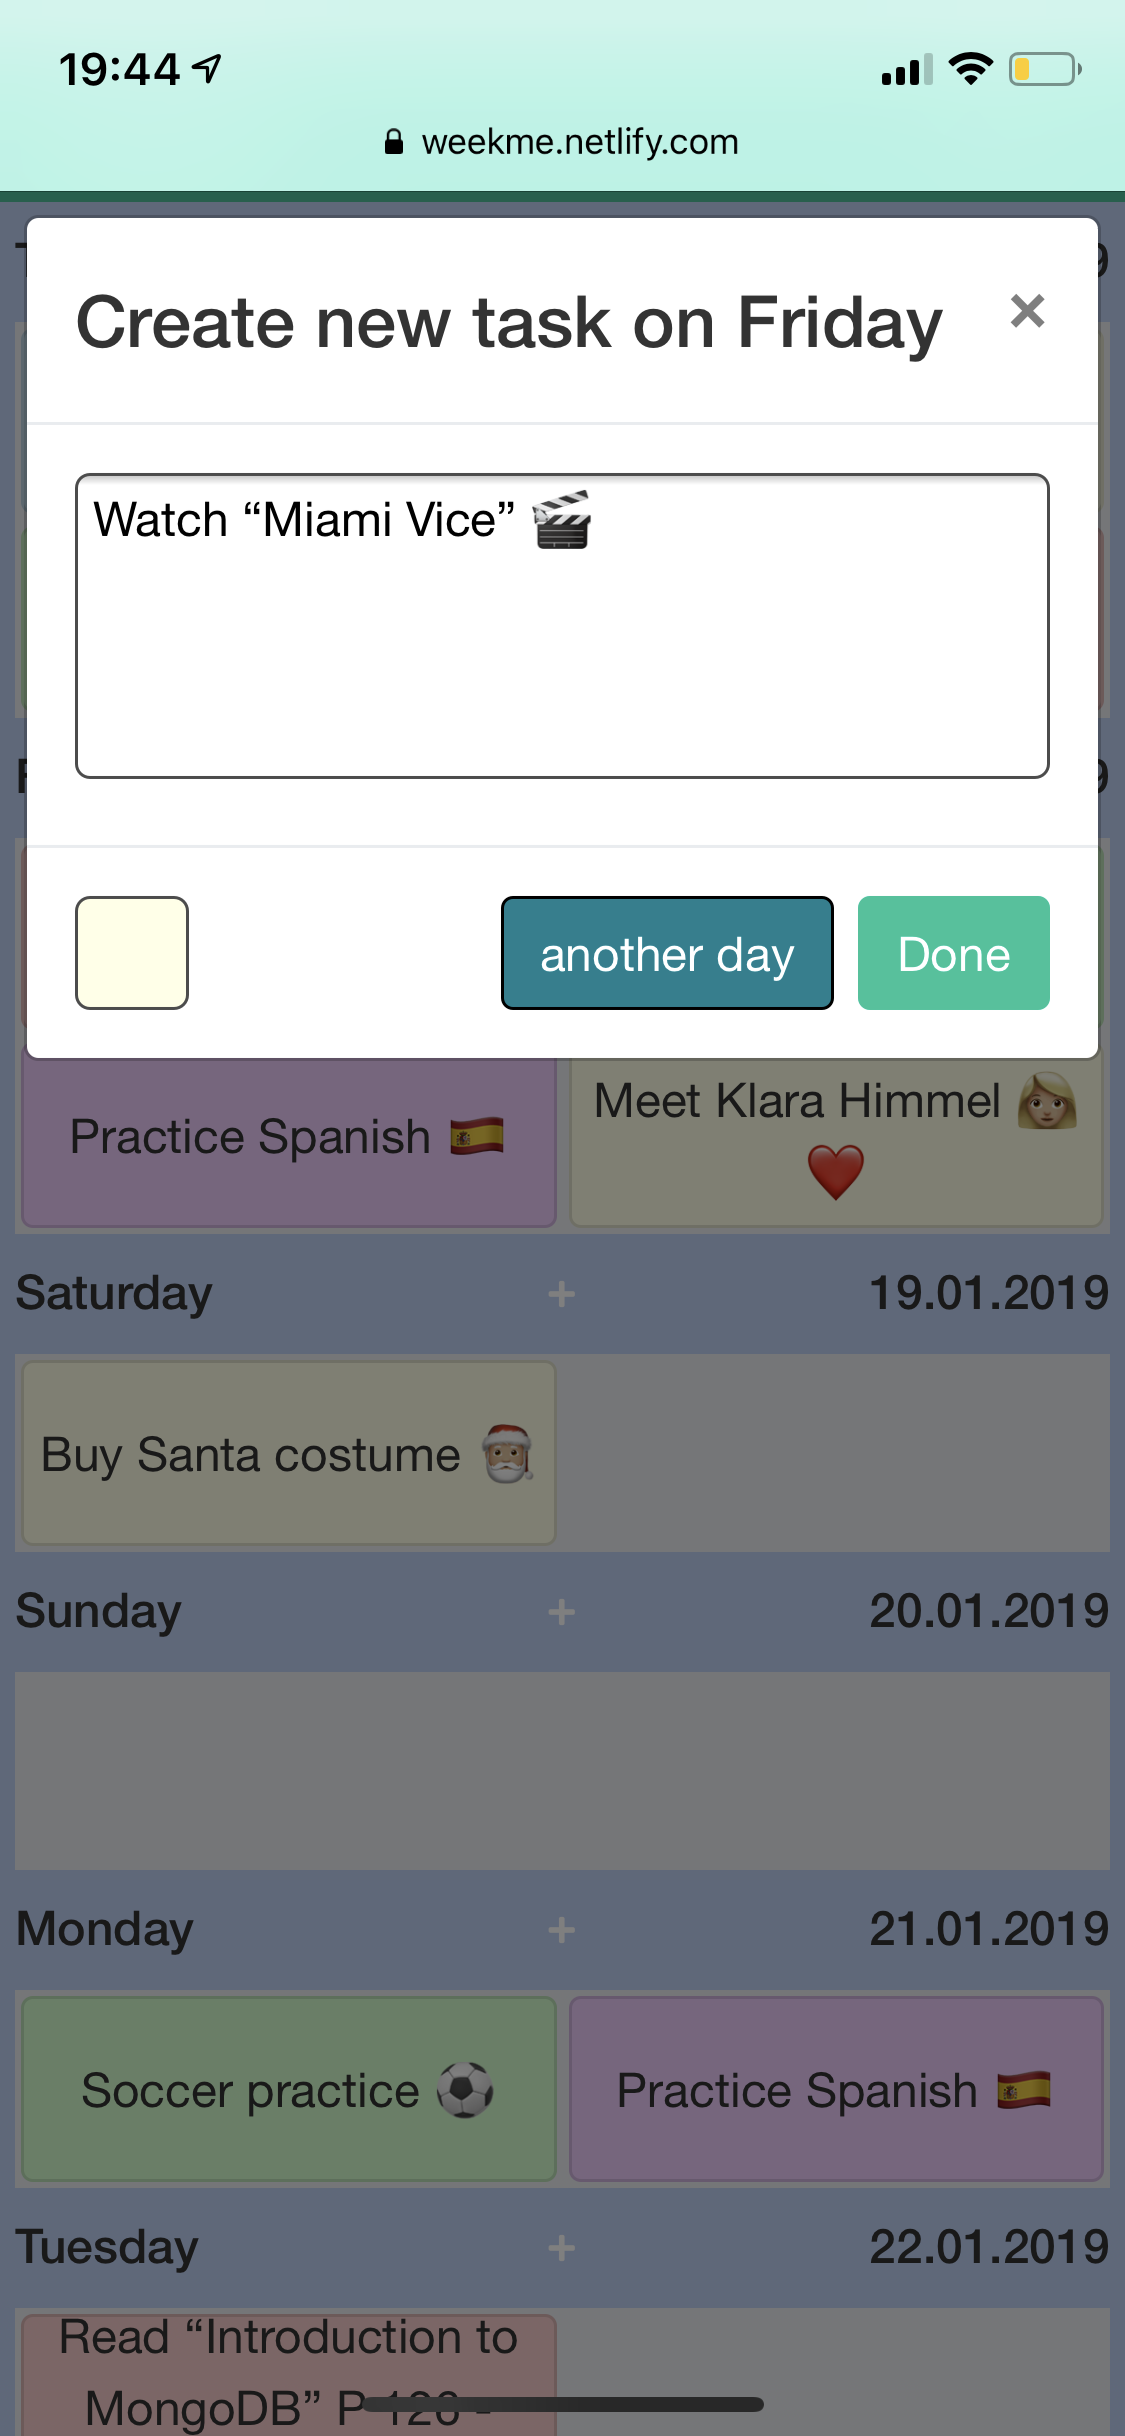
\includegraphics[height=10cm]{figures/user_docu_createtask.PNG} }}
    \qquad
    \subfloat[Change day later on]{{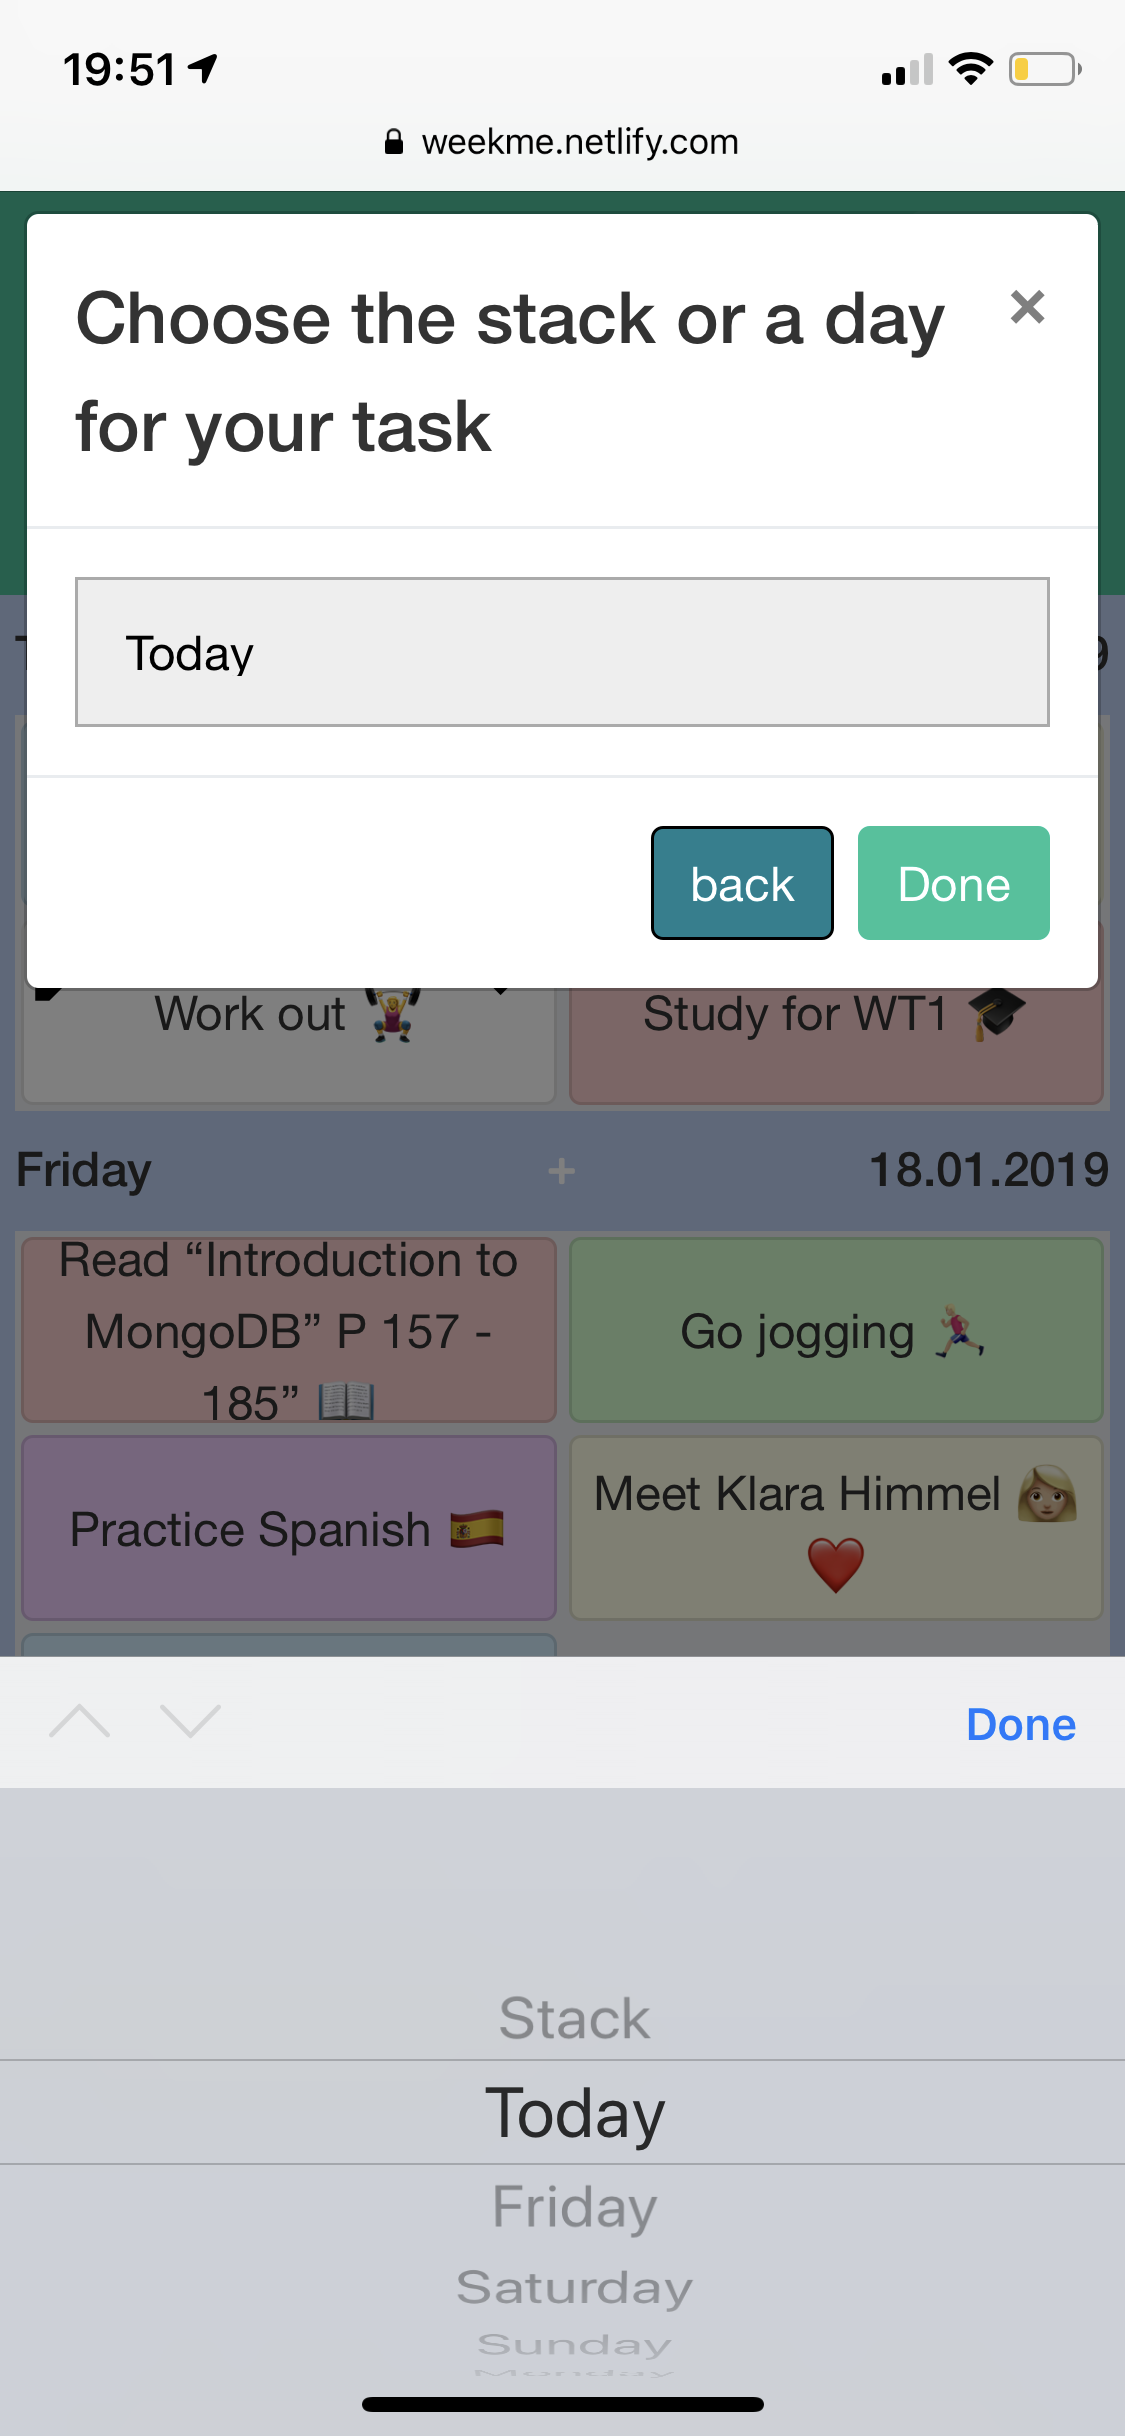
\includegraphics[height=10cm]{figures/user_docu_createtask_day.PNG} }}
    \caption{Creation process on mobile}
    \label{fig:example}
\end{figure}
 
\subsubsection{Editing tasks}
In case you misspelled something, you want to rephrase something or you just have too much colour on your screen and want to make changes to a task you previously created, just select the task by clicking/tapping on it and select the handy edit button in the upper left corner. 
\subsubsection{Moving tasks}
If you want to bring tasks within one day into order, you can move them around! Just select a task and select the task you want to swap positions with afterwards. 
This also works if you want to move a task to a different day. 
\subsubsection{Checking off and deleting tasks}
You did it. You successfully planned something, stuck to the plan and finished a task. What do you do now? You check the task off by selecting it and clicking/tapping the checkmark icon in the top right corner. It's really that easy! \\
Don't like a task you created anymore? Just check it off as done - no one will know!

\begin{figure}[H] 
	\centering 
	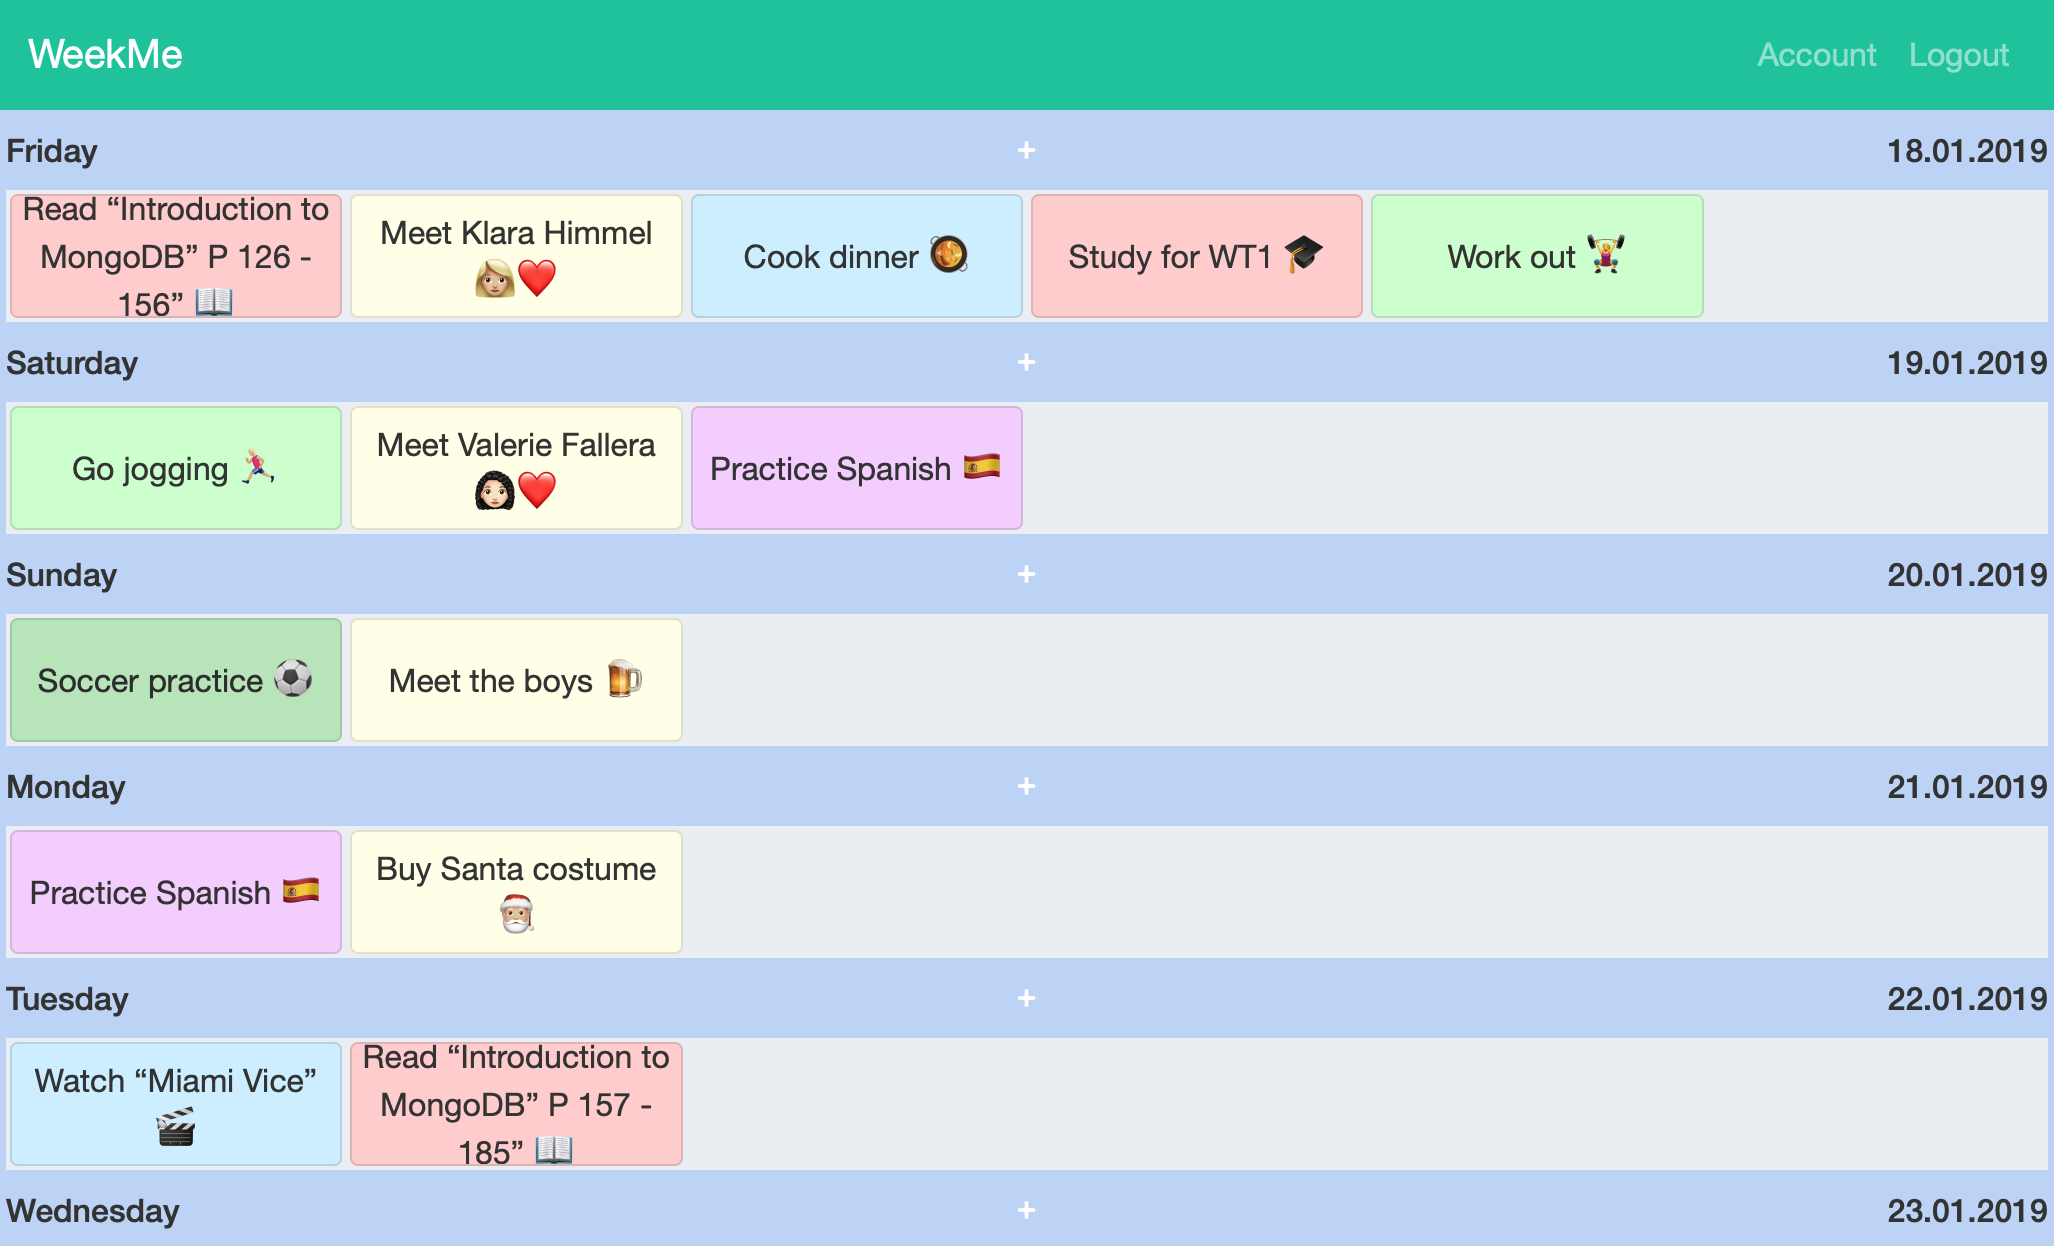
\includegraphics[width=14cm]{figures/user_docu_selected_task_desktop.png}   
	\caption[WeekMe account page]{When selecting a task two buttons will appear}       
	\label{fig: Selected task on desktop}     
\end{figure}  

\subsubsection{The stack} 
At the very bottom of your week there is an eighth entry labeled "stack" - What's that all about you might ask - well, this is where you can put tasks that you know you want to do but just don't exactly know when.  You can interact with it just as with every other day as explained above.  
In case you did not manage to check off everything on any given day those tasks will automatically be moved to the stack for you.

\subsubsection{Task creation workflow}
Step by step description on how to create a task. 

	\begin{figure}[H] 
		\centering 
		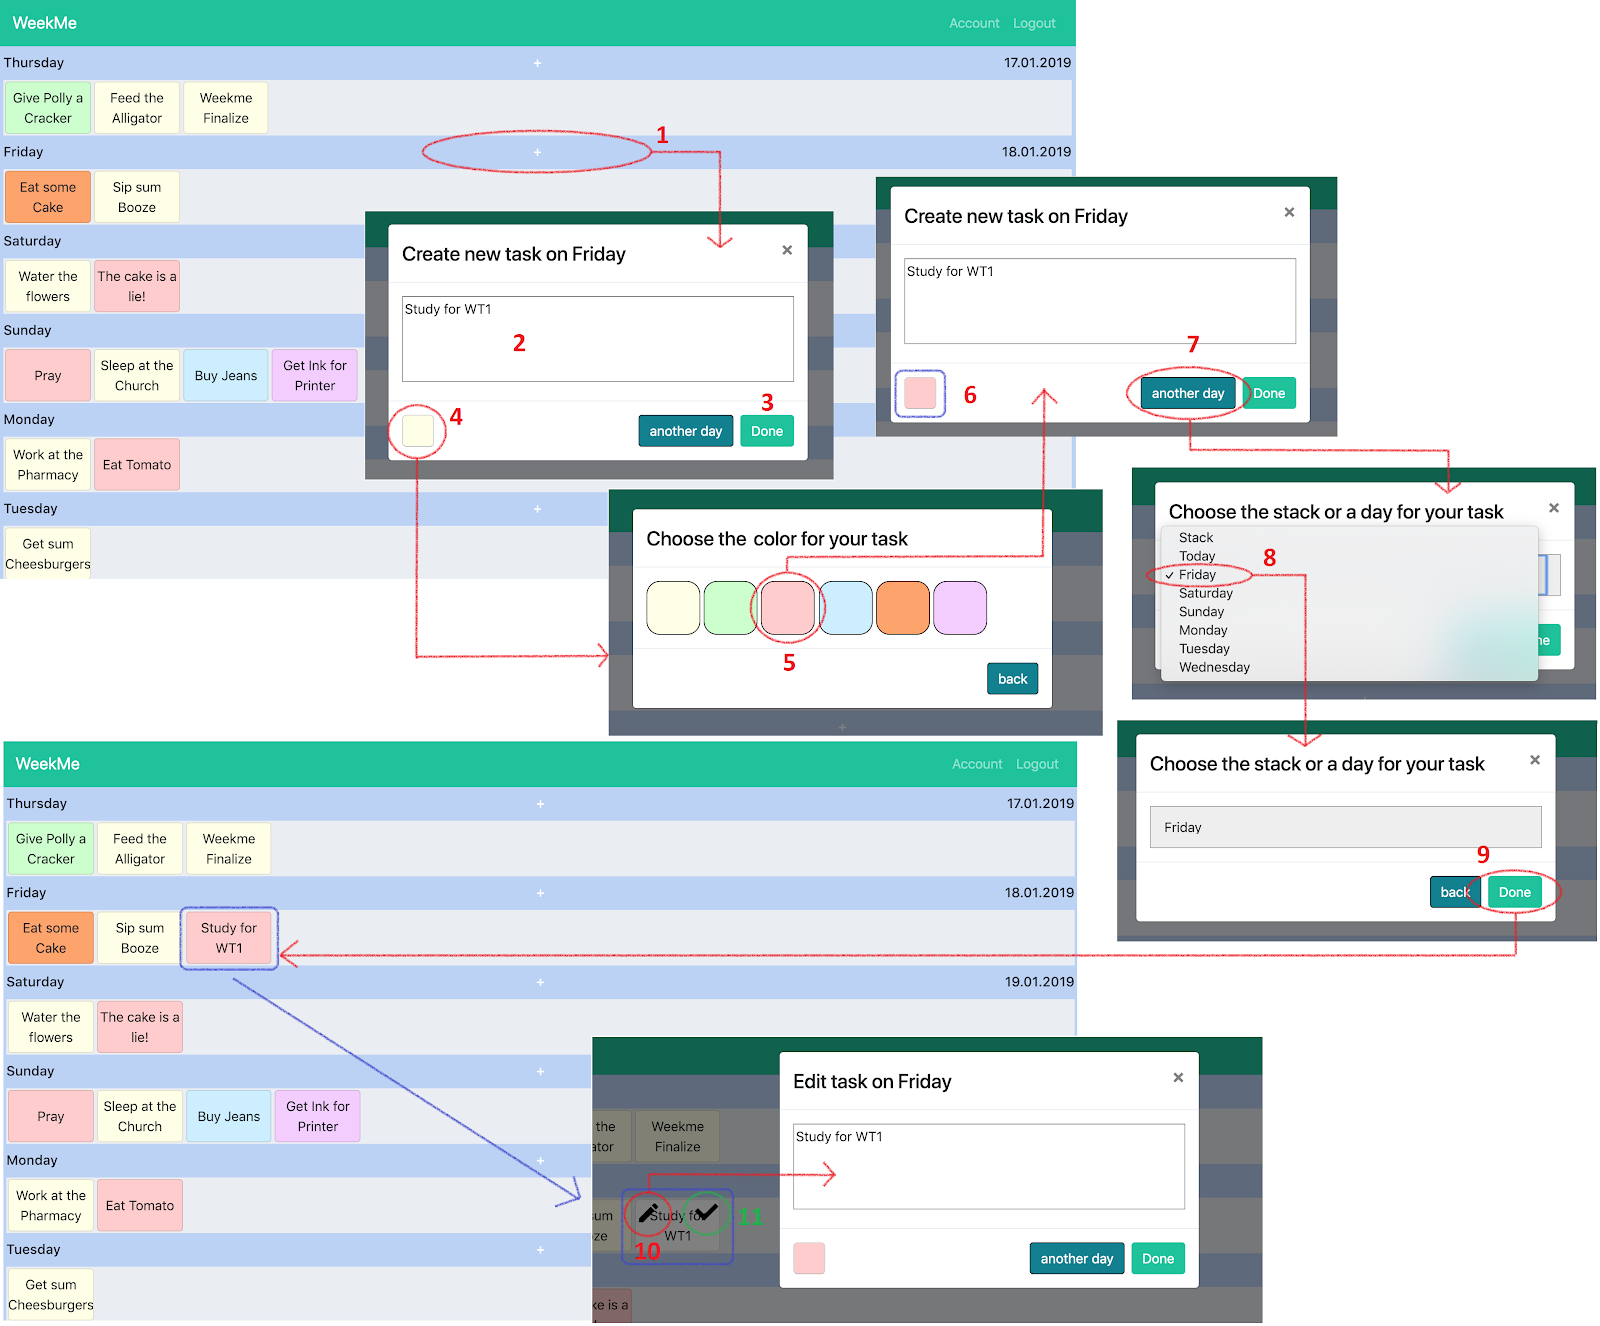
\includegraphics[height=12cm]{figures/task_creation_workflow}    
		\caption[Task creation workflow]{Task creation workflow}     
		\label{fig: Task creation workflow}     
	\end{figure}  
\newpage	
\begin{enumerate}
	\item Click on one of the seven pluses (+) to start the process to create a new task in the corresponding day. 
	\item A popup window will open where you can enter a task-description.
	\item Now you can finish the process by clicking the done button (the task will be added to the day container with the default color (light-yellow). 
	\item Optionally you can click the coloured button on the left to open the colour-picker.
	\item Choose a color for your task by clicking it or press back. 
	\item Step one will be shown again with an updated color in the colour-picker-button.
	\item Now you can modify your description, finish the creation-process or change the day the task will be added to by clicking “another day”.
	\item In this case just choose the day you wish out of a dropdown-menu.
	\item Press “Done” to finish or “Back” if you want to reach step one again to modify your task.
	\item If you want to edit an existing task just click on the task and afterwards on the small pen symbol.
	\item If you click on the check symbol of a task you will finish and delete the task.
\end{enumerate}
